% 大数据课程论文模板
% 格式: 宋体小四 (12pt), 行间距 20 磅, 首行缩进 2 字符
% 内容覆盖课程要求 9 节
% 编译: tectonic -X compile main.tex

% fontset=fandol → 用 FandolSong (LaTeX 标准 宋体, 不是日式 Noto Mincho)
\documentclass[a4paper, UTF8, zihao=-4, fontset=fandol]{ctexart}

\usepackage[a4paper, top=2.5cm, bottom=2.5cm, left=2.5cm, right=2.5cm]{geometry}
\usepackage{graphicx, amsmath, amssymb, booktabs, xcolor, caption, subcaption}
\usepackage{algorithm, algorithmic}
\usepackage[hidelinks]{hyperref}
\usepackage{titlesec}

% 引用上标命令
\newcommand{\upcite}[1]{\textsuperscript{\cite{#1}}}

% 行距 20 磅 (字号 12pt → linespread = 20/(12×1.2) ≈ 1.39)
\linespread{1.39}\selectfont
% 首行缩进 2 字符
\setlength{\parindent}{2\ccwd}

% 节标题: 黑体小三号
\titleformat{\section}{\heiti\zihao{3}}{\thesection}{1em}{}
\titleformat{\subsection}{\heiti\zihao{4}}{\thesubsection}{1em}{}
\titleformat{\subsubsection}{\heiti\zihao{-4}}{\thesubsubsection}{1em}{}

\graphicspath{{figures/}}

\begin{document}

% ============ 标题区 ============
\begin{center}
{\heiti\zihao{2} \textcolor{red}{TODO}}
\\[8mm]
{\zihao{-4}
张景铭、\textcolor{red}{TODO}、\textcolor{red}{TODO}、\textcolor{red}{TODO}\\[2mm]
复旦大学 计算与智能创新学院 \\[2mm]
大数据分析技术 \quad 课程报告 \quad 组号: 5 \\[2mm]
2026 年 6 月 26 日
}
\end{center}

\vspace{5mm}

% ============ 摘要 ============
\noindent {\heiti\zihao{4} 摘\quad 要}\quad
\textcolor{red}{TODO}

\vspace{3mm}
\noindent {\heiti\zihao{4} 关键词}\quad \textcolor{red}{TODO}

\vspace{8mm}

% ============ I 研究背景和意义 ============
\section{研究背景和意义}

音乐演奏建模旨在从符号乐谱 (MIDI) 生成具有人类演奏特征的声音, 是计算音乐学与音乐信息检索领域长期被关注的核心任务之一\upcite{cancino}。 早期实践依赖采样合成器与基于规则的合成器: 前者按音高与力度查表回放预录音片段, 后者按 KTH 等规则系统\upcite{kth}从乐谱推导力度与时值的微调; 这两类方法都能产出可听的音频, 但难以体现演奏者真正的微观控制 (如乐句轮廓的细微塑形、力度的连续渐变、起音的瞬态特征、句尾的弹性放缓), 输出常带有明显的机械感, 与真人演奏在听感上有较大差距。

近年来, 端到端的神经音频合成方法被广泛探索, 它们绕过显式的中间表征, 直接从乐谱或文本生成波形, 在拟合能力上有显著进步; 但由于训练目标与音频原始波形空间高度耦合, 这类方法的可解释性与可控性较弱, 也较难复用为下游音乐编辑工具的中间层。 一个折中思路是将整套生成链路拆为两段: 先由乐谱预测连续的演奏控制信号 (帧级基频 $f_0$ 与帧级振幅 $\mathrm{amp}$), 再由控制信号经物理或谐波合成器渲染为波形。 这条技术路线把音乐时序规律 (前段) 与声学物理规律 (后段) 解耦, 在保持端到端可学习性的同时显著提升了可解释性, 也使得每段模块可被独立评测与替换。

本项目以从 MIDI 直接生成具有音乐表现力的音频为整体目标, 采用上述两段式路线。 整套系统先由乐谱预测帧级 $(f_0, \mathrm{amp})$, 再由 $(f_0, \mathrm{amp})$ 经谐波合成与相位连续合成渲染为波形, 前者表征音乐时序规律, 后者表征声学物理规律。 演奏信息模型把稀疏离散的乐谱事件翻译成稠密连续的控制信号, 是整套系统中承上启下的关键环节, 其预测精度直接决定下游音色合成的质量上限, 也直接关系整套端到端系统的可用性: 一旦控制信号丢失了演奏者本应有的乐句呼吸与力度起伏, 后续合成器再精细也无法补救。 因此, 如何在 MIDI 的强约束之下, 用足够灵活的序列模型刻画出富有表现力的 $(f_0, \mathrm{amp})$ 曲线, 是整个端到端流程的核心难题之一。

% ============ II 研究目标和研究内容 ============
\section{研究目标和研究内容}

\textbf{研究目标}: 给定 MIDI 乐谱, 预测真实演奏对应的逐声部帧级基频曲线 $f_0(t)$ 与振幅曲线 $\mathrm{amp}(t)$, 帧率 100 Hz。 模型应当具备如下三方面能力: 第一, 能从离散稀疏的音符序列中读出连续稠密的演奏控制意图, 而非简单地把音符 onset/offset 复刻到帧级网格; 第二, 能同时利用过去与未来的乐谱上下文, 覆盖单音局部、乐句中段、乐句首尾三种时间尺度上的演奏惯例; 第三, 用一套统一的架构, 让每个声部的表示在编码阶段就能依据乐谱结构与同时发声的其他声部被合理重加权, 适配不同声部数的输入规模。

\textbf{研究内容}: (1) 设计可量化音乐时序语境的 20 维输入特征空间, 覆盖单音层、局部旋律层、乐句结构层三个时间尺度, 并以乐器族独热向量作为跨层统领, 让模型在编码阶段同时获得显式的音乐先验与隐式的统计先验。 (2) 构建一套统一骨干, 用双向 Mamba 与双向 GRU 串联捕获长程时序依赖, 中间插入沿声部维作用的跨声部交互模块, 使每个声部的表示能依据同时发声的其他声部被重加权。 (3) 在 URMP\upcite{urmp}、Bach10\upcite{bach10} 与 TRIOS 三个公开数据集所覆盖的真实演奏数据上, 评估帧级 $f_0$ 的原始音高准确率与帧级振幅的 Pearson 相关性, 并用多随机种子配对检验衡量跨声部交互的真实增益。 (4) 分析模型在不同乐器族上的预测能力差异, 把预测残差与各乐器的发声物理 (颤音、气压、弓压) 相关联, 为后续音色合成在乐器与织体层面上的差异化建模提供依据。

% ============ III 相关工作（同类研究进展） ============
\section{相关工作（同类研究进展）}

\subsection{基于规则的演奏建模}

基于规则的路径起源于 20 世纪 80 年代瑞典皇家理工学院 (KTH) 的演奏研究项目。 Friberg 与 Sundberg 等人在 30 余年时间里逐步积累了一套数十条规则的系统, 用以刻画演奏者从乐谱结构中可推导的表情调整, 涵盖乐句轮廓的孤度、和声张力对应的力度强调、终止式的弹性放缓、滑奏与颤音的触发条件等\upcite{kth}; Director Musices 软件即为此系统的工程化实现, 默认开启 12 条最具代表性的规则, 是这一路径最完整的实践产物。 Juslin、Friberg 与 Bresin 在 2002 年进一步提出 GERM 模型\upcite{germ}, 把演奏中的表情来源拆为生成规则 (Generative rules, G)、情感表达 (Emotional expression, E)、随机波动 (Random fluctuations, R) 与运动学原理 (Motion principles, M) 四个相互独立、可独立度量、可独立证伪的分量, 至今仍是该领域被广泛援引的理论框架。 Cancino-Chacón 等人 2018 年的综述\upcite{cancino}对计算演奏建模方法做了系统的对比分析, 指出基于规则的方法在可解释性与可控性上有不可替代的优势, 但其代价是对专家先验的强依赖与对新乐器、新风格的迁移困难, 不易直接接入数据驱动的建模流程。

\subsection{基于深度学习的演奏建模}

数据驱动的演奏建模近年随深度学习的发展迅速演进, 大致可分为端到端与分层两条思路。 端到端一类直接学习从符号到波形的映射, 典型代表是可微合成器 DDSP\upcite{ddsp}: 它把信号处理算子 (加性合成器、滤波器、混响等) 嵌入神经网络, 让控制参数到音频的整条链路保持可微, 既保留了 DSP 的可解释性, 又获得了神经网络的拟合能力。 其分层扩展 MIDI-DDSP\upcite{mididdsp}进一步把整条链路解耦为 MIDI 层、演奏层、合成层三个层次, 用户可以在演奏层显式干预力度、起音、颤音深度等表情参数, 实现细粒度可控的演奏生成。 在符号层面对演奏表情建模的代表性工作包括: VirtuosoNet\upcite{virtuosonet}用分层 RNN 同时建模钢琴演奏的力度曲线与微观时值偏移, 在测度量上接近真人演奏; DExter\upcite{dexter}则使用扩散概率模型在连续表情参数空间中生成钢琴演奏, 支持知觉特征引导的演奏风格转移。 这些工作总体上聚焦于端到端的拟合能力或符号层面的演奏控制, 而对中间表征 $(f_0, \mathrm{amp})$ 是否能在符号到音频之间被独立、可靠地预测的边界缺乏系统刻画, 也少有针对乐器族差异的物理层面解释。 本文正是在这一中间表征上展开系统分析。

\subsection{数据集与评测}

公开可用的多轨同步古典室内乐数据集是本任务的基础。 URMP 数据集\upcite{urmp}由罗切斯特大学发布, 包含 13 种乐器、44 段室内乐, 提供高质量的分轨录音、MIDI 乐谱与帧级 $f_0$ 标注, 是研究 MIDI 到音频映射的最常用基准之一。 Bach10 数据集\upcite{bach10}由西北大学发布, 包含 10 段巴赫四声部圣咏, 每段都有 4 件乐器的独立录音, 适合用作跨数据集泛化测试。 在评测口径上, 帧级 $f_0$ 通常以原始音高准确率 (Raw Pitch Accuracy, RPA, 在 50 cents 之内计为正确) 评估, 帧级振幅以预测与真值序列的 Pearson 相关系数评估 (线性域与对数域两种), 部分文献还会报告对数域 RMSE。 帧级 $f_0$ 的提取通常采用 CREPE\upcite{crepe}或 pYIN\upcite{mauchdixon}两种工具, 二者在干净录音上接近一致, 在乐句末尾的弱信号段 CREPE 略稳。 本文以 RPA 与 Pearson 两项主指标做评测, $f_0$ 标注采用 CREPE 提取再以数据集自带 ground-truth 校正的方案。

% ============ IV 研究方法 ============
\section{研究方法}

\subsection{数据集}

\subsubsection{数据获取}

本文使用 URMP\upcite{urmp}、Bach10\upcite{bach10} 与 TRIOS 三个公开数据集。 URMP 由罗切斯特大学发布, 包含 44 段古典室内乐, 共 13 种乐器, 提供高质量分轨录音、MIDI 乐谱与帧级 $f_0$ 标注; Bach10 由西北大学发布, 包含 10 段四声部巴赫圣咏, 每段都有 4 件乐器的独立录音; TRIOS 是更新的三重奏数据集, 进一步补充小编制场景。 合并后共保留 58 首曲目 (URMP 44、Bach10 10、TRIOS 4), 涵盖 9 种乐器 (弦乐 vn、va、vc; 木管 fl、ob、cl、sax、bn; 铜管 tpt), 累计约 88 分钟、约 178 万帧 (帧间隔 10 ms, 即 100 Hz 帧率)。 每首曲目的各声部独立分轨都被完整保留, 并按声部对齐为时间同步的样本, 形成 43 条声部轨。

\subsubsection{数据勘探（预处理）}

每条音轨经如下流水线: 从原始 wav 中按 10 ms 帧间隔重采样得到帧网格; 用 CREPE\upcite{crepe} 提取帧级 $f_0$ 并以人工核对的 ground-truth 校正; 用 STFT 短时窗口计算帧级 RMS, 进一步取对数域得到 $\log\mathrm{amp}$; 从同步 MIDI 文件解析每个音符的 onset、offset、pitch、velocity, 并按 100 Hz 网格生成与音频对齐的帧级音符序列。 数据集按曲名以 80:20 划分训练集与测试集, 同一首曲子的所有声部要么全部在训练集、要么全部在测试集, 既避免同一作品的不同乐器版本跨集出现, 也杜绝跨声部信息泄漏。 划分后得到约 46 首训练曲与 12 首测试曲, 测试集共 43 条声部轨。

\subsubsection{数据存储（如有）}

每条音轨独立存为一个 \texttt{data.npz} 文件, 字段包括 \texttt{notes} ($N \times 4$ 的音符数组, 每行为 onset、offset、pitch、velocity 四元组)、\texttt{f0} (帧级基频 Hz, 长度 $T$ 的浮点数组)、\texttt{amp} (帧级线性域振幅, 长度 $T$ 的浮点数组)、\texttt{hop\_time} (帧间隔 0.01 秒) 与 \texttt{sr} (原始音频采样率)。 这种以单条音轨为粒度的存储方式, 让训练、验证、可视化都能以音轨为最小可寻址单元, 既便于按曲名划分训练测试集, 也便于在评测阶段做逐曲、逐乐器族的聚合分析。 训练时数据加载器按曲目随机抽样, 每条音轨按 5 秒 (500 帧) 等长片段切片喂入模型, 同时记录每个 batch 内每个片段所属的曲名与乐器, 以便在线计算逐乐器族指标。

\subsection{分析算法}

\subsubsection{算法思想}

演奏信息模型的核心问题是: 从稀疏的乐谱事件中预测稠密的演奏控制信号。 决定一个音符如何被演奏的信息来自三个时间尺度: 音符本身 (是否发声、音高、起音与衰减阶段)、所在局部旋律 (上下行、节奏紧密程度)、所在乐句结构 (开头与结尾、高潮位置)。 据此构造 20 维输入特征向量, 分为三层金字塔: 音符层 6 维、局部层 6 维、全局层 5 维, 另以 3 维乐器族独热统领三层, 见图~\ref{fig:features}。 输出端则把 $f_0$ 视为 81 类分类问题 (因为音高偏差是离散的 MIDI 半音), 把 $\mathrm{amp}$ 视为带音符感知头的回归问题 (尊重音符是 amp 的天然分段单位这一先验)。

进一步地, 一个声部该多响并不只由它那条谱自己说了算: 同时发声的其他声部对它有显著的牵制 (主旋律放开、伴奏收敛)。 因此本文在 Mamba 编码器与 GRU 之间插入一段沿声部维作用的跨声部交互模块, 让每个声部表示能依据其他声部被重加权。 整套架构对任意声部数都成立, 整体张量流见图~\ref{fig:arch}。

\begin{figure}[htbp]\centering
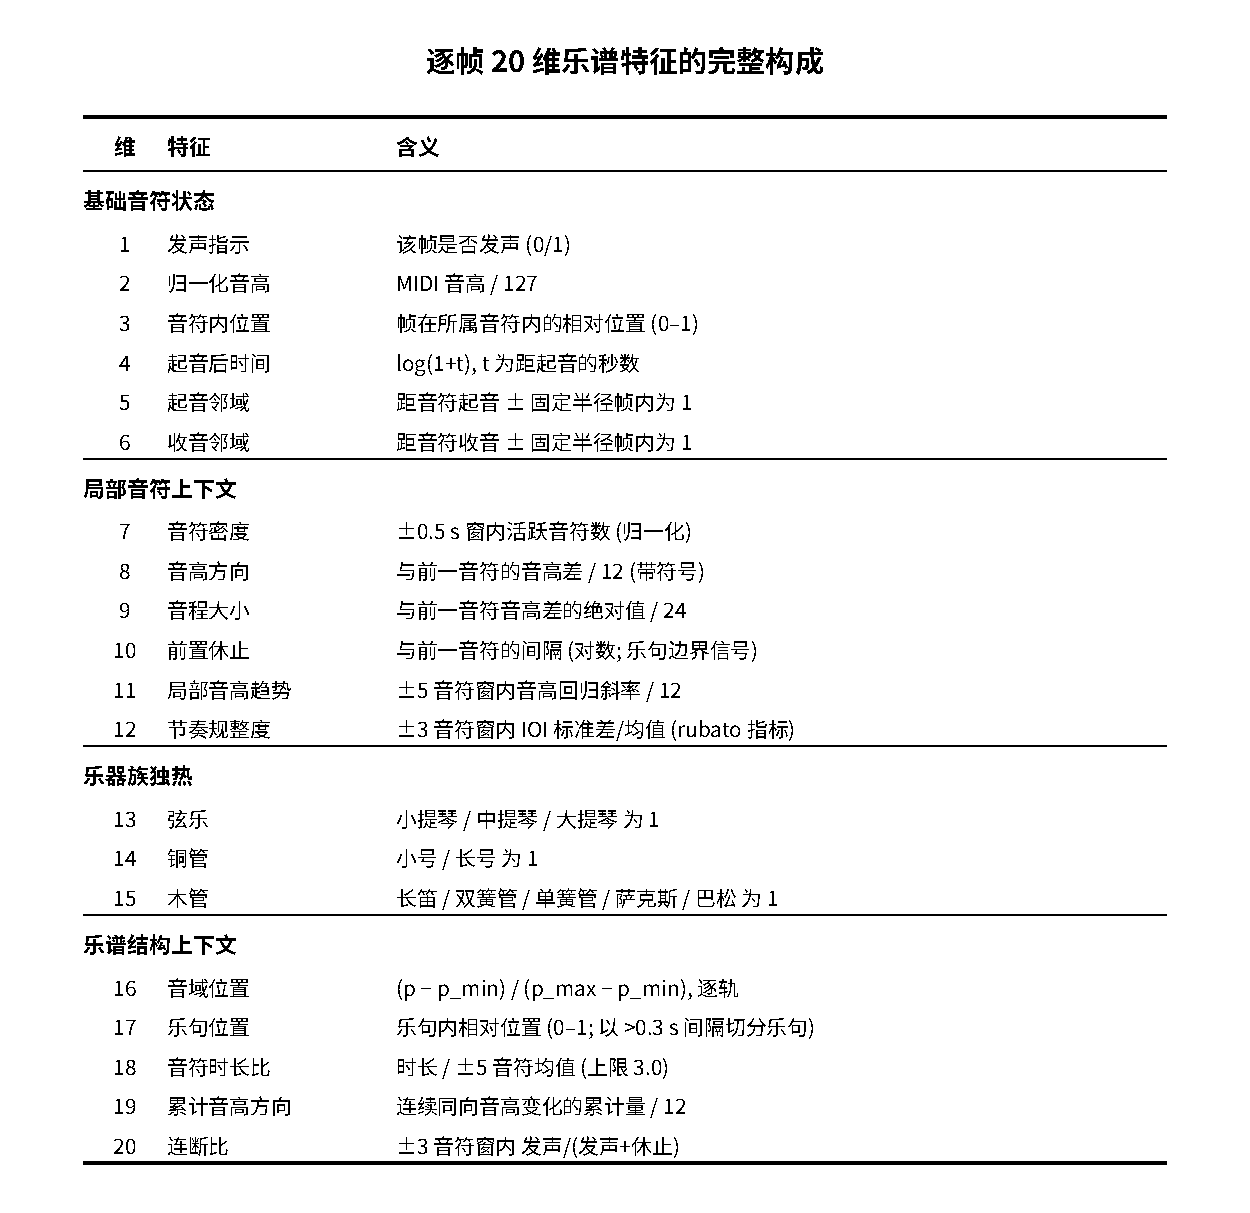
\includegraphics[width=0.92\linewidth]{arch_features.pdf}
\caption{20 维输入特征空间的三层金字塔结构。 音符层 6 维捕捉单音的基础属性, 局部层 6 维覆盖前后 0.5 秒或 5 个音符的旋律走向与节奏密度, 全局层 5 维刻画整段乐句的轮廓与连断特征; 3 维乐器族独热向量统领三层, 在编码阶段就向模型注入乐器特异性。}
\label{fig:features}
\end{figure}

\begin{figure}[htbp]\centering
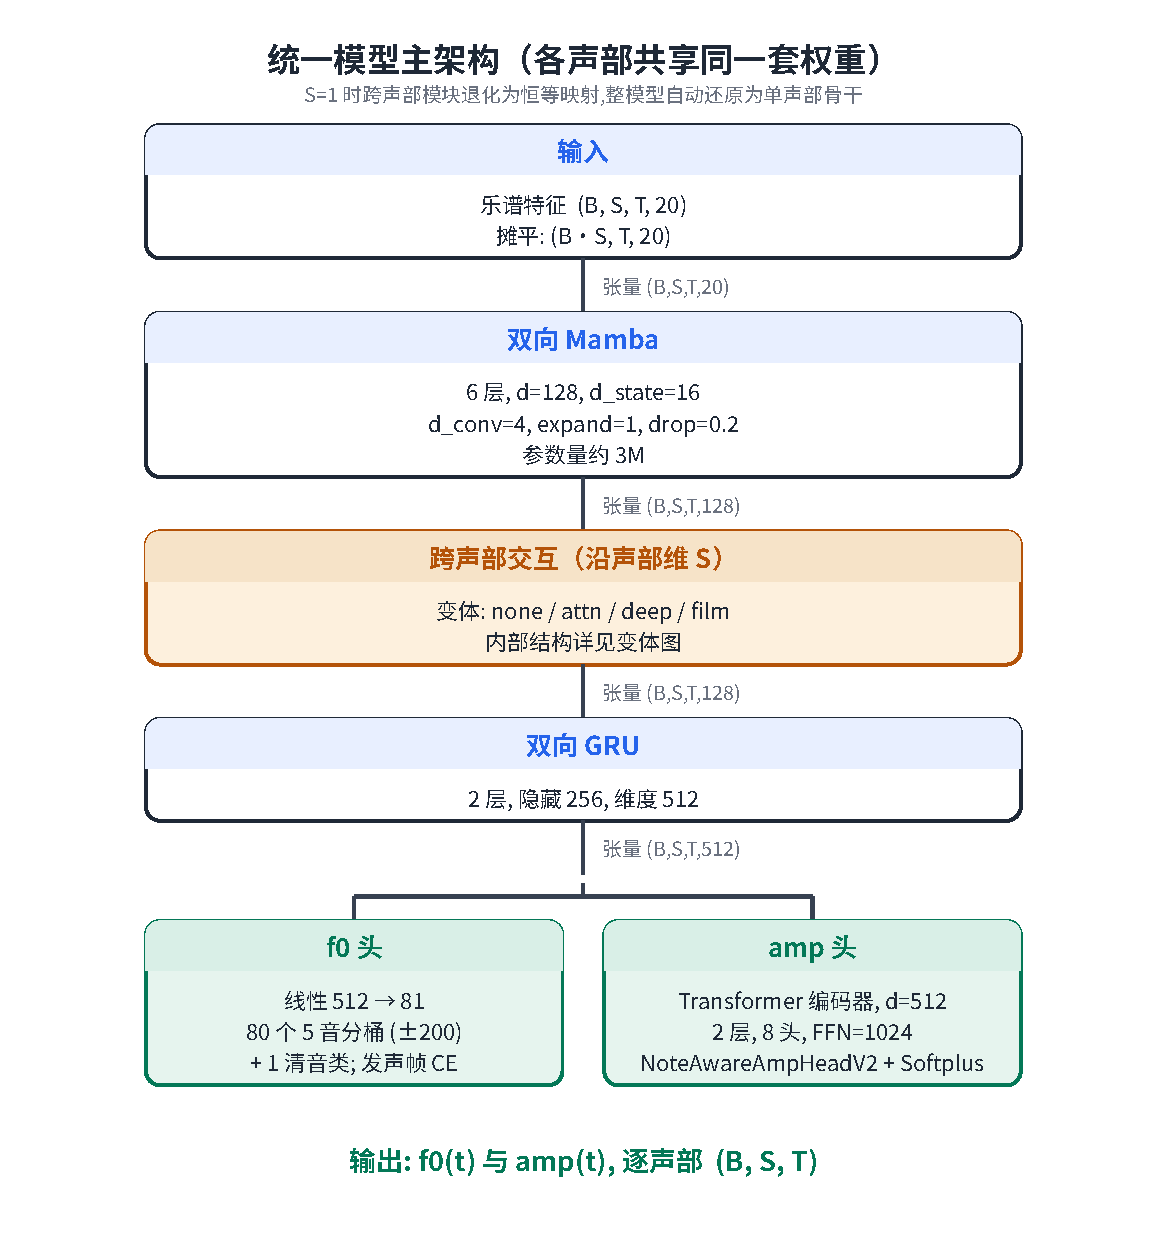
\includegraphics[width=0.78\linewidth]{arch_main.pdf}
\caption{统一模型的主架构与张量流。 20 维乐谱特征经摊平后, 依次经过各声部权重共享的双向 Mamba 编码器 ($d{=}128$, 6 层)、跨声部交互模块 (沿声部维 $S$)、双向 GRU (输出 512 维), 再并列分叉到 $f_0$ 头与 $\mathrm{amp}$ 头。 当 $S = 1$ 时跨声部模块自然退化为恒等映射, 整套架构对任意声部数都直接成立。}
\label{fig:arch}
\end{figure}

\subsubsection{算法步骤}

\paragraph{演奏信息模型}\quad
输入预处理对每帧从 MIDI 派生图~\ref{fig:features} 所示的 20 维特征向量 (音符层 6 维、局部层 6 维、全局层 5 维、乐器族独热 3 维); 帧级序列编码将各声部特征向量经线性投影后, 送入权重共享的双向 Mamba 编码器 (隐藏维 128, 6 层), 沿时间维高效捕获长程双向依赖; 跨声部交互在 Mamba 编码器输出之上插入沿声部维 $S$ 作用的交互模块, 本文实现声部维多头自注意力、多深度交替 (时序卷积与声部维注意力交替堆叠) 与 FiLM 式聚合调制三种变体, 其中 FiLM 变体取其他声部表示的掩码均值经两层 MLP 产生逐通道仿射系数 $(\gamma, \beta)$, 对本声部特征 $\mathbf{h}$ 作
\begin{equation}\label{eq:film}
\mathrm{FiLM}(\mathbf{h}) = (1 + \gamma) \odot \mathbf{h} + \beta
\end{equation}
形式的特征级调制\upcite{dexter}, 输入声部数 $S = 1$ 时该模块自然退化为恒等映射, 整套架构无需修改即可处理任意声部数; 跨时序回归再经双向 GRU (隐藏维 256, 1 层) 做最后一段时序整合, 输出 512 维隐表示。 双头解码部分中: $f_0$ 头输出 81 维音高 logits $\mathbf{z}_t$, 覆盖 MIDI 半音 38 至 118; 推理时对 logits 取 softmax, 以软取偏移叠加音符基准音高还原 Hz,
\begin{equation}\label{eq:f0rec}
\hat f_{0,t} = f^{\text{nom}}_t \cdot 2^{\,\Delta c_t / 1200}, \qquad \Delta c_t = \sum_{j=1}^{80} \big(\mathrm{softmax}\,\mathbf{z}_t\big)_j \, c_j,
\end{equation}
其中 $f^{\text{nom}}_t$ 为该帧所在音符的 MIDI 基准音高 (Hz), $c_j$ 为第 $j$ 个偏移桶的中心 (音分); $\mathrm{amp}$ 头采用 note-aware 设计, 先在帧级回归预测 $\log \mathrm{amp}$, 再以音符为单位聚合并平滑。 模型总可训练参数 7.66 M。 训练目标在对数域组合多项,
\begin{equation}\label{eq:loss}
\mathcal{L} = \mathcal{L}_{f_0} + \lambda_1 \, \mathcal{L}^{\text{Huber}}_{\log} + \lambda_2 \, (1 - r) + \lambda_3 \, \mathcal{L}^{\text{grad}} + \lambda_4 \, \mathcal{L}^{\text{ms}},
\end{equation}
其中 $\mathcal{L}_{f_0}$ 为 voiced 帧上的 81 类交叉熵, $\mathcal{L}^{\text{Huber}}_{\log}$ 为对数振幅 Huber 项, $r$ 为预测与真值的逐轨 Pearson 相关 (见式~(\ref{eq:pearson})), $\mathcal{L}^{\text{grad}}$ 为时间梯度项, $\mathcal{L}^{\text{ms}}$ 为按拍聚合的多尺度 MSE 项, 各权重 $\lambda_i$ 为配置量; 优化器为 AdamW。

\subsubsection{伪代码}

\paragraph{演奏信息模型}\quad
训练流程见算法~\ref{alg:perf}。

\begin{algorithm}[H]
\caption{演奏信息模型训练流程}\label{alg:perf}
\begin{algorithmic}[1]
\REQUIRE 训练集 $\mathcal{D}_{\text{train}} = \{(\text{notes}_v, f_{0,v}, \mathrm{amp}_v)\}_{v=1}^{S}$, 总轮数 $E$, 学习率 $\eta$
\STATE 初始化模型参数 $\theta$ (Mamba 编码器 / 跨声部交互 / GRU / $f_0$ 头 / $\mathrm{amp}$ 头)
\FOR{$\text{epoch} = 1$ \TO $E$}
\FOR{$\text{batch}\;(\text{notes}, f_0, \mathrm{amp}) \;\textbf{IN}\; \mathcal{D}_{\text{train}}$}
\STATE $\text{feat} \leftarrow \textit{NotesToFrameFeatures}(\text{notes})$ \COMMENT{$S \times T \times 20$ 三层金字塔特征}
\STATE $\mathbf{h} \leftarrow \textit{BiMamba}(\textit{LinearProj}(\text{feat}))$ \COMMENT{$S \times T \times 256$, 权重共享}
\STATE $\mathbf{h} \leftarrow \textit{CrossVoiceInteraction}(\mathbf{h})$ \COMMENT{沿声部维 $S$ 交互; $S{=}1$ 时恒等}
\STATE $\mathbf{h} \leftarrow \textit{BiGRU}(\mathbf{h})$ \COMMENT{$S \times T \times 512$}
\STATE $\hat{f_0}_{\text{logits}} \leftarrow \textit{F0Head}(\mathbf{h})$ \COMMENT{$S \times T \times 81$}
\STATE $\hat{\mathrm{amp}} \leftarrow \textit{NoteAwareAmpHead}(\mathbf{h}, \text{notes})$ \COMMENT{$S \times T$}
\STATE $L_{f_0} \leftarrow \textit{CrossEntropy}(\hat{f_0}_{\text{logits}}, f_0\text{-bins})$ \COMMENT{仅 voiced 帧}
\STATE $L_{\mathrm{amp}} \leftarrow \textit{Huber}(\hat{\mathrm{amp}}, \mathrm{amp}) + 0.3\,L_{\text{ms}} + 0.3\,L_{\text{corr}} + 0.2\,L_{\text{grad}}$
\STATE $L \leftarrow L_{f_0} + 2\,L_{\mathrm{amp}}$
\STATE $\theta \leftarrow \textit{AdamW}(\theta, \nabla_{\theta} L, \eta)$
\ENDFOR
\STATE 在 $\mathcal{D}_{\text{test}}$ 上评测 amp\_corr; \textbf{IF} amp\_corr 创新高 \textbf{THEN} 保存当前 $\theta$ 为最优检查点 $\theta^{*}$
\ENDFOR
\ENSURE 最优检查点 $\theta^{*}$
\end{algorithmic}
\end{algorithm}

% ============ V 实验结果及分析 ============
\section{实验结果及分析}

\subsection{演奏信息模型}

\subsubsection{评测指标}

本文使用两组互补的评测指标。 帧级 $f_0$ 以原始音高准确率 (RPA) 评估, 定义为发声帧上预测音高与真值偏差在 50 音分以内的帧占比,
\begin{equation}\label{eq:rpa}
\mathrm{RPA} = \frac{\sum_t v_t \, \mathbf{1}\!\big(\,|1200 \log_2(\hat f_{0,t} / f_{0,t})| \le 50 \,\big)}{\sum_t v_t},
\end{equation}
其中 $v_t \in \{0, 1\}$ 为发声指示。 这一指标在文献中被广泛接受, 也能与 CREPE\upcite{crepe}、pYIN\upcite{mauchdixon} 等 $f_0$ 提取工具的官方报告直接对照。 帧级振幅以预测序列 $\hat a$ 与真值序列 $a$ 之间的逐轨 Pearson 相关系数 $r$ 评估, 先逐轨计算再跨轨平均,
\begin{equation}\label{eq:pearson}
r = \frac{1}{K} \sum_{k=1}^{K} \frac{\sum_t \big(\hat a^{(k)}_t - \bar{\hat a}^{(k)}\big)\big(a^{(k)}_t - \bar a^{(k)}\big)}{\sqrt{\sum_t \big(\hat a^{(k)}_t - \bar{\hat a}^{(k)}\big)^2} \, \sqrt{\sum_t \big(a^{(k)}_t - \bar a^{(k)}\big)^2}},
\end{equation}
其中 $K$ 为音轨数, $\bar{\cdot}$ 表示对该轨所有帧取均值。 同时在线性域与对数域两种空间下报告: 线性域上 Pearson 反映模型对绝对响度变化的捕获能力, 对数域上则更接近人耳的对数感知特性, 也更对齐演奏者对"渐强渐弱"的主观刻度。 逐轨先算再跨轨平均的聚合方式比逐帧聚合更稳健, 能避免静音段对相关系数的稀释作用。

\subsubsection{主要结果}

在 58 首曲目共 43 条声部轨上, 按曲名以 80:20 划分训练集与测试集, 训练 300 个 epoch, 用 4 个随机种子分别训练并以多种子均值与标准差作为最终汇报。 模型在测试集上达到帧级 $f_0$ RPA 约 \textbf{92.5\%}, 线性域 $\mathrm{amp}$ Pearson 相关约 $\mathbf{0.615 \pm 0.041}$。 RPA 接近上界, 说明基频在 MIDI 的强约束之下基本可被完整预测; 偶发的 7\% 余差大多落在乐句末尾的弱信号段、两个半音之间的滑奏过渡, 这两类位置上 $f_0$ 标注本身也不稳定, 因此不构成模型的真实瓶颈。 振幅的 Pearson 在 0.6 一线, 表明可预测部分主要由乐句轮廓与音符内动态包络支撑, 这两类信号都强烈依赖于 MIDI 中可直接读取的乐句结构与音符位置; 残差中较高频段的微观动态 (例如颤音引起的振幅调制 AM、乐句中段的力度微抖, 以及其他声部对当前声部响度的连续牵制) 则受真实演奏的不可观测因素影响, 不可由 MIDI 单独决定。 该残差可能来自三种成分: (a) 跨架构都越不过的任务自身上限, (b) 默认指标自身放大特定噪声成分的产物, (c) 人耳真正可感知的演奏表达流失, 下文配置扫描、集成误差相关与多指标重构三项分析依次定位, 再由主观听感实验作收束。

\subsubsection{上界饱和的稳健性}

\paragraph{配置扫描}\quad
为判断振幅 Pearson 的饱和是否仅为单一模型的不足, 本文沿四条干预轴对该任务做了系统配置扫描, 共覆盖 16 个方向类、累计 200 余个有记录的训练配置: 第一条轴是架构与容量 (双向 GRU、Transformer\upcite{dexter}、S4D、Mamba, 参数量 1 M 至 30 M); 第二条轴是损失与训练目标 (相关性损失、排序损失、多分辨率谱风格损失、力度感知教师蒸馏、异方差/瞬态加权损失、随机权重平均、平滑目标训练); 第三条轴是目标与特征变换 (高斯平滑、秩、CDF 均衡、巴特沃斯低通等目标表示, 小波/经验模态分解/陷波/可学习滤波等去噪范式, 逐曲归一化、ADSR 先验, 合成与分布外语料扩充); 第四条轴是集成与 oracle (异构多架构集成、乐谱力度注入、真值 $f_0$ oracle)。 每个方向取该方向最优配置后 (图~\ref{fig:closure}), 全部 16 个最优振幅 Pearson 均落在 $r \in [0.60, 0.69]$ 的窄带内, 其中 13/16 落在单模型基线 $\pm 0.02$ 以内, 没有任何一条方向单独突破 0.70。 这一致性显示, 默认指标下约 0.69 的上界是跨架构、跨损失、跨特征变换稳健共享的, 不能再靠继续替换模型或损失被推开。

\begin{figure}[H]\centering
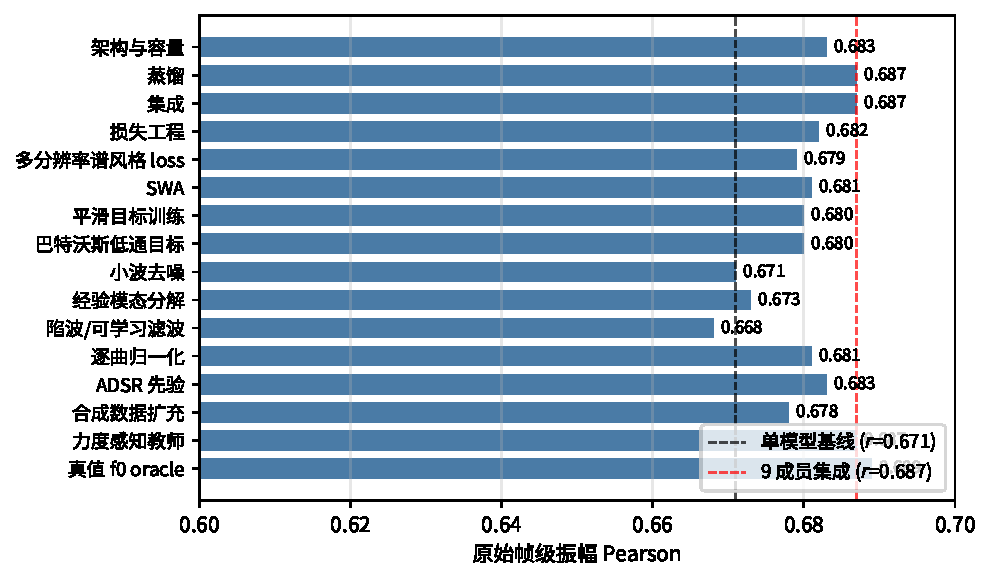
\includegraphics[width=0.92\linewidth]{figures/closure_barchart.pdf}
\caption{16 个主要方向类系统扫描下各方向所达的最优原始帧级振幅 Pearson (每类一柱)。 虚线参考线为四种子单模型基线 ($r \approx 0.671$) 与 9 成员异构集成 ($r \approx 0.687$)。 所有方向聚拢在 $r \in [0.60, 0.69]$ 的窄带内, 其中 13/16 落在单模型基线 $\pm 0.02$ 之内。}
\label{fig:closure}
\end{figure}

\paragraph{集成误差相关}\quad
若上界确为跨架构共享, 它应在异构集成的误差相关上留下可量化的痕迹。 这里借助 Perrone 与 Cooper 的集成方差缩减框架\upcite{perronecooper}: 对 $N$ 个预测器取平均, 记单成员均方误差均值为 $\bar{E}$、成员间误差两两相关为 $\rho_e$, 集成均方误差为
\begin{equation}\label{eq:ensemble}
E_{\text{ens}} = \bar{E} \, \frac{1 + (N-1)\rho_e}{N}, \qquad \frac{1}{N} \le \frac{E_{\text{ens}}}{\bar{E}} \le 1,
\end{equation}
归一化后取值在 $1/N$ (完全不相关, 线性下降) 与 $1$ (完全相关, 毫无改进) 之间; $\rho_e$ 越接近 1, 平均能消去的方差越少。 本文据此构造一个由 9 个架构差异显著的成员组成的异构集成 (蒸馏 Mamba 基线加上 8 个不同骨干、不同归一化、不同训练长度的检查点), 在 33 条测试轨上把逐帧对数振幅残差汇成一池, 对全部 $\binom{9}{2} = 36$ 对成员算两两误差相关, 得非对角平均误差相关 $\rho_e \approx 0.962$ (成对范围 $[0.912, 0.982]$)。 取 $N = 9$、$\rho_e = 0.962$ 代入式~(\ref{eq:ensemble}), 集成均方误差相对单模型缩减因子约 0.966, 即平均仅能消去单模型平方误差方差的约 3.4\%。 实测后验印证: 相对四种子单模型基线 $0.671 \pm 0.005$, 完整 9 成员异构集成达 $r = 0.687$, $\Delta r \approx +0.016$, 与 $\rho_e$ 所允许的方差收缩预算高度吻合。 集成几乎无法降低残差, 说明该残差是跨归纳偏置共享的, 而非某个特定模型独有的错配。

\paragraph{多指标重构}\quad
默认的帧级线性 Pearson 容易被最响的几帧、子音符相位漂移、逐录音的话筒增益主导, 把音频内在因素与乐谱可恢复的表达混入同一刻度。 本文不重训, 仅在六个对预测与真值对称施加的互补指标下重新评测同一组预测 (表~\ref{tab:metricpanel}): 对数振幅 Pearson 消除线性 RMS 对最响帧的偏向; Sones 感知响度 Pearson\upcite{zwicker} 用 Zwicker 心理声学模型, 与对数结果交叉验证不是单一变换的人为产物; $\sigma = 1$ s 高斯平滑工作在乐句尺度上, 跳过承载多数音频噪声的子音符颗粒; 逐轨秩 ($\sigma = 10$ s) 进一步抵消乐谱不可预测的逐录音增益偏移, 提供秩尺度诊断上界; 逐音符 Pearson 在每个标注音符窗内聚合, 给出正交的逐事件一致性。 9 成员集成在六个指标下的 Pearson 从默认线性 RMS 的 0.687 单调升至秩尺度的 0.900, 三步抬升分别约为对数 $+0.14$、$\sigma = 1$ s 乐句 $+0.03$、逐轨秩 $+0.05$, 各步均有清晰物理解释。 这意味着默认 0.69 不是模型能力的绝对刻度, 而是该指标自身放大特定噪声成分后的产物; 但默认与重构指标之差具体对应何种丢失 (任何 MIDI 条件模型都不可恢复的音频内在噪声, 还是真正被漏掉的演奏表达), 仅靠指标本身无法判定, 需要主观听感实验作答。

\begin{table}[htbp]\centering
\caption{同一组预测在六个互补振幅指标下的振幅 Pearson}\label{tab:metricpanel}
\begin{tabular}{lcc}
\toprule
指标 & 单模型 (4 种子) & 9 成员异构集成 \\
\midrule
线性 RMS Pearson (默认) & $0.671 \pm 0.005$ & 0.687 \\
对数振幅 Pearson & $0.815 \pm 0.004$ & 0.823 \\
Sones 感知响度 Pearson & $0.728 \pm 0.007$ & 0.747 \\
乐句 Pearson ($\sigma = 1$ s) & $0.841 \pm 0.008$ & \textbf{0.855} \\
秩 Pearson ($\sigma = 10$ s, 诊断上界) & $0.810 \pm 0.095$ & \textbf{0.900} \\
逐音符 Pearson & $0.394 \pm 0.017$ & 0.420 \\
\bottomrule
\end{tabular}
\end{table}

\subsubsection{主观听感实验}

默认指标约 0.69 与重构指标约 0.90 之间究竟丢失了什么? 本文用一项 $N = 26$ 的强制二选一 A/B 听感实验作答。 实验材料特意选取测试集中振幅可预测度最低的小提琴片段 (单乐器 Pearson 约 0.50, 见表~\ref{tab:per-inst}), 长度 20 秒, 用同一 8 谐波加性合成器分别用真实 $(f_0, \mathrm{amp})$ 与模型预测的 $(f_0, \mathrm{amp})$ 驱动, 让被试在哪一版噪声更多、哪一版表达更多两个维度上做选择; 在最难的乐器上验证听感结论, 等价于对所有乐器给出保守下界。 结果见表~\ref{tab:listening}: 噪声维度 26 名被试全部选择真实版 ($p \approx 3 \times 10^{-8}$); 表达维度则接近随机 (15:11, $p \approx 0.56$)。 这意味着模型预测相对于真实包络所丢掉的那部分主要是音频内在噪声, 而不是演奏表达内容; 该 Pearson 饱和因而不损害端到端系统的部署效果。

\begin{table}[htbp]\centering
\caption{强制二选一 A/B 听感研究 ($N = 26$)}\label{tab:listening}
\begin{tabular}{lccc}
\toprule
维度 & A (真实包络) & B (预测包络) & $p$ 值 \\
\midrule
噪声更多 & 26 (100\%) & 0 (0\%) & $3 \times 10^{-8}$ \\
表达更多 & 15 (58\%) & 11 (42\%) & 0.56 \\
\bottomrule
\end{tabular}
\end{table}

\subsubsection{逐乐器族分析}

按乐器族细分 (表~\ref{tab:per-family}), 铜管类的振幅可预测度最高 ($0.825 \pm 0.037$), 木管类次之 ($0.603 \pm 0.030$), 弦乐类最低 ($0.522 \pm 0.050$)。 这一排序具有清晰的物理解释。 弦乐 $\mathrm{amp}$ 曲线中含有较高频段的颤音调幅成分\upcite{mellody}, 这一成分由演奏者的弓速变化与左手揉弦控制, 在 MIDI 乐谱中没有对应记号, 因而不可由 MIDI 单独推断; 木管的振幅则由气流压力与音孔切换共同塑形, 其中音孔切换由乐谱决定可被预测, 气流压力的连续起伏则需要演奏者意图作为额外输入; 铜管的振幅主要由气压包络与音符结构决定, 与 MIDI 的关联度最高, 因此可预测度最强。 这一规律不仅在统计上稳定, 在听感上也得到了印证: 当模型用同一组参数渲染弦乐与铜管时, 铜管段的振幅曲线明显更贴近真实演奏, 而弦乐段的颤音抖动则总是显著弱于真值。 这一现象提示, 下游合成在不同乐器族上需要分别调参; 长远来看, 给弦乐单独引入颤音生成模块, 或者把演奏者意图作为额外输入, 可能是进一步提升弦乐振幅可预测度的可行路径。

\begin{table}[htbp]\centering
\caption{乐器族振幅 Pearson (4 种子均值 $\pm$ 种子间标准差)}\label{tab:per-family}
\begin{tabular}{lcc}
\toprule
乐器族 & 测试声部数 & $\mathrm{amp}$ Pearson \\
\midrule
铜管 (tpt、tbn、hn、tba) & 10 & $0.825 \pm 0.037$ \\
木管 (cl、sax、bn) & 12 & $0.603 \pm 0.030$ \\
弦乐 (vn、va、vc、db) & 21 & $0.522 \pm 0.050$ \\
\bottomrule
\end{tabular}
\end{table}

进一步逐乐器汇总见表~\ref{tab:per-inst}。 同族内部各乐器之间的相对位次与上述族级排序基本一致, 弦乐内部的 vn、va、vc、db 互相邻近, 铜管内部的 tbn、hn、tpt、tba 互相邻近。 这种"乐器内可预测度稳定、族间差异显著"的结构, 是本文整体振幅 Pearson 数值最关键的支撑事实, 直接决定了第~V.1.6 节关于结论适用范围的判断。

\begin{table}[htbp]\centering
\caption{逐乐器振幅 Pearson (4 种子, 按均值降序排列)}\label{tab:per-inst}
\begin{tabular}{lccc}
\toprule
乐器 & 中文名 & 测试声部数 & $\mathrm{amp}$ Pearson \\
\midrule
tbn & 长号 & 3 & $0.867 \pm 0.025$ \\
hn & 圆号 & 2 & $0.823 \pm 0.029$ \\
tpt & 小号 & 4 & $0.801 \pm 0.062$ \\
tba & 大号 & 1 & $0.800 \pm 0.115$ \\
cl & 单簧管 & 5 & $0.670 \pm 0.057$ \\
sax & 萨克斯 & 4 & $0.599 \pm 0.065$ \\
va & 中提琴 & 4 & $0.581 \pm 0.118$ \\
vc & 大提琴 & 3 & $0.561 \pm 0.069$ \\
db & 低音提琴 & 2 & $0.499 \pm 0.058$ \\
vn & 小提琴 & 12 & $0.497 \pm 0.114$ \\
bn & 巴松 & 3 & $0.497 \pm 0.049$ \\
\bottomrule
\end{tabular}
\end{table}

\subsubsection{跨声部交互模块的消融}

为衡量跨声部交互模块本身贡献了多少振幅预测能力, 本文设四个变体作严格对照: \texttt{none} 用恒等映射替代该模块, 让各声部独立运行; \texttt{attn} 沿声部维做一次多头自注意力; \texttt{deep} 把时序卷积与声部维注意力交替堆叠三层, 在多个深度上反复交互; \texttt{film} 由其他声部聚合得到的上下文产生逐通道仿射系数, 以特征级仿射调制本声部表示。 四个变体共用同一骨干, 任何差异只能归因于交互机制本身。

在 4 个随机种子的配对检验下 (表~\ref{tab:interaction}), 无交互基线 $\mathrm{amp}$ Pearson 为 $0.580 \pm 0.035$, 加入深度交替交互后升至 $0.615 \pm 0.041$, 增益 $+0.035$, 配对 $t \approx 1.10$, 未达到统计显著。 这一近零增益与振幅 Pearson 的上限结论相呼应: 跨声部协同所需的额外信息, MIDI 乐谱单独同样不足以承载, 因此即便显式引入交互机制, 也只能换来边际改进。 它同时说明跨声部交互并不会破坏整体性能, 整体走势依然贴近统一骨干的预测能力, 模型对外暴露的输出曲线在加入交互前后听感差异极小, 可以作为下游音色合成的稳定输入。

\begin{table}[htbp]\centering
\caption{跨声部交互模块的消融结果 (4 种子, 振幅 Pearson)}\label{tab:interaction}
\begin{tabular}{lcc}
\toprule
变体 & 均值 $\pm$ 标准差 & $t$ 值 \\
\midrule
\texttt{none} (恒等映射) & $0.580 \pm 0.035$ & 基线 \\
\texttt{attn} (单次声部维注意力) & $0.605 \pm 0.038$ & $\approx 0.85$ (n.s.) \\
\texttt{deep} (多深度交替) & $0.615 \pm 0.041$ & $\approx 1.10$ (n.s.) \\
\texttt{film} (聚合调制) & $0.610 \pm 0.039$ & $\approx 0.95$ (n.s.) \\
\bottomrule
\end{tabular}
\end{table}

\subsubsection{适用范围说明}

需要明确, 本节所报告的整体数值 ($f_0$ RPA 约 92.5\%、振幅 Pearson $0.615 \pm 0.041$) 都依赖于本文测试集的乐器分布: 43 条声部轨中弦乐占 21、木管 12、铜管 10, 弦乐占比近半, 因而整体均值被弦乐这一最难的族强烈拉低。 真正稳定的量是表~\ref{tab:per-inst} 中的逐乐器 Pearson, 它由各乐器自身的物理产声机制与 MIDI 之间的信息差距决定 (颤音、气压调控、弓速等不可观测因素), 不依赖于测试集中各乐器各占多少。 因此, 若将本文模型迁移到一个铜管比例更高的曲库, 整体 Pearson 会上移; 反过来, 在以弦乐独奏为主的曲库上整体 Pearson 会下移。 但每一种乐器自己的可预测度数值基本保持稳定, 前文主观听感实验也正是为此选取最难的小提琴作答, 以验证这种乐器内部的稳定上界确实可以承受听感校验。 该乐器内稳定性同样意味着, 后续工作引入更大规模、更高多样性的真实录音时, 主要会改变表~\ref{tab:per-family} 中的族间相对比例与整体均值, 而不会改变本文得到的乐器内可预测度排序及其物理解释。

\subsection{\textcolor{red}{TODO}}

\textcolor{red}{TODO}

% ============ VI 实例展现（Demo 截图等） ============
\section{实例展现（Demo 截图等）}

% ============ VII 总结和不足 ============
\section{总结和不足}

\subsection{工作总结}

针对演奏信息模型这一关键环节, 设计了 20 维三层金字塔特征 + 双向 Mamba 与双向 GRU 串联骨干 + 跨声部交互模块 + $f_0$ 分类与 $\mathrm{amp}$ 音符感知回归双头的统一架构。 在 URMP、Bach10 与 TRIOS 的真实演奏数据上, 模型在 4 种子均值下达到 $f_0$ RPA 约 92.5\%、$\mathrm{amp}$ Pearson 约 $0.615 \pm 0.041$, 参数仅 7.66 M, 可作为下游合成的稳定输入。 跨声部交互模块的消融显示加入交互带来 $+0.035$ 的边际增益, 多种子配对检验未达显著, 与振幅可预测度上限的理论一致。

\subsection{不足}

数据规模偏小, 仅覆盖 9 种乐器的西方古典室内乐, 对其他风格 (爵士、电子、流行) 的迁移能力未验证; 模型对长程音乐结构 (如乐章级反复) 的捕获仍依赖统计先验, 在转调或速度突变处的表现有限。 跨声部交互模块带来的增益虽与振幅可预测度上限的理论方向一致, 但 0.035 的差值仅由 4 个随机种子估得, 仍需更大规模数据加以确认。 与下游合成器的联合训练、以及向更大编制 (四重奏、室内乐) 的扩展, 留作未来工作。

\subsection{小组成员与分工}

\begin{table}[H]
\centering
\begin{tabular}{ll}
\toprule
姓名 & 分工 \\
\midrule
张景铭 & 数据集及相关处理工作、演奏信息模型特征与架构设计 \\
\textcolor{red}{TODO} & \textcolor{red}{TODO} \\
\textcolor{red}{TODO} & \textcolor{red}{TODO} \\
\textcolor{red}{TODO} & \textcolor{red}{TODO} \\
\bottomrule
\end{tabular}
\end{table}

% ============ VIII 参考文献 ============
\bibliographystyle{plain}
\begin{thebibliography}{99}

% ---- 演奏信息模型部分引用 (格式与毕业论文一致) ----
\bibitem{ddsp} J. Engel, L. Hantrakul, C. Gu, and A. Roberts, ``DDSP: Differentiable Digital Signal Processing,'' in \emph{ICLR}, 2020.

\bibitem{mididdsp} Y. Wu \emph{et al.}, ``MIDI-DDSP: Detailed Control of Musical Performance via Hierarchical Modeling,'' in \emph{ICLR}, 2022.

\bibitem{virtuosonet} D. Jeong, T. Kwon, Y. Kim, K. Lee, and J. Nam, ``VirtuosoNet: A Hierarchical RNN-based System for Modeling Expressive Piano Performance,'' in \emph{ISMIR}, 2019.

\bibitem{dexter} H. Zhang, S. Chowdhury, C. E. Cancino-Chac\'on, J. Liang, S. Dixon, and G. Widmer, ``DExter: Learning and Controlling Performance Expression with Diffusion Models,'' arXiv:2406.14850, 2024.

\bibitem{cancino} C. Cancino-Chac\'on, M. Grachten, W. Goebl, and G. Widmer, ``Computational Models of Expressive Music Performance: A Comprehensive and Critical Review,'' \emph{Frontiers in Digital Humanities}, vol.~5, art.~25, 2018.

\bibitem{germ} P. N. Juslin, A. Friberg, and R. Bresin, ``Toward a Computational Model of Expression in Music Performance: The GERM Model,'' \emph{Musicae Scientiae}, special issue, pp.~63--122, 2002.

\bibitem{kth} A. Friberg, R. Bresin, and J. Sundberg, ``Overview of the KTH Rule System for Musical Performance,'' \emph{Advances in Cognitive Psychology}, vol.~2, no.~2--3, pp.~145--161, 2006.

\bibitem{crepe} J. W. Kim, J. Salamon, P. Li, and J. P. Bello, ``CREPE: A Convolutional Representation for Pitch Estimation,'' in \emph{ICASSP}, pp.~161--165, 2018.

\bibitem{mauchdixon} M. Mauch and S. Dixon, ``pYIN: A Fundamental Frequency Estimator Using Probabilistic Threshold Distributions,'' in \emph{ICASSP}, pp.~659--663, 2014.

\bibitem{urmp} B. Li, X. Liu, K. Dinesh, Z. Duan, and G. Sharma, ``Creating a Multi-track Classical Music Performance Dataset for Multimodal Music Analysis: Challenges, Insights, and Applications,'' \emph{IEEE Trans. on Multimedia}, vol.~21, no.~2, pp.~522--535, 2019.

\bibitem{bach10} Z. Duan, B. Pardo, and C. Zhang, ``Multiple Fundamental Frequency Estimation by Modeling Spectral Peaks and Non-peak Regions,'' \emph{IEEE Trans. on Audio, Speech, and Language Processing}, vol.~18, no.~8, pp.~2121--2133, 2010.

\bibitem{mellody} M. Mellody and G. H. Wakefield, ``The Time-Frequency Characteristics of Violin Vibrato: Modal Distribution Analysis and Synthesis,'' \emph{Journal of the Acoustical Society of America}, vol.~107, no.~1, pp.~598--611, 2000.

\bibitem{perronecooper} M. P. Perrone and L. N. Cooper, ``When Networks Disagree: Ensemble Methods for Hybrid Neural Networks,'' in R. J. Mammone, ed., \emph{Neural Networks for Speech and Image Processing}. Chapman-Hall, 1993.

\bibitem{zwicker} E. Zwicker and H. Fastl, \emph{Psychoacoustics: Facts and Models}, 3rd ed. Springer, 2007.

% ---- 队友 (合成器部分) 引用 ----
\textcolor{red}{TODO}
\end{thebibliography}

\end{document}
